% Figure 3 of the thesis (cohort flow, p.20). The tikzpicture below is copied unchanged from the thesis source
% (Chapter 2, figure label fig:cohort_flow), where it is drawn inline. For standalone compilation the preamble
% loads the TikZ libraries of the thesis and defines \citep so that the two citations print as in the thesis.
% Compile: pdflatex fig_3_cohort_flow.tex
\documentclass[12pt,border=1pt]{standalone}
\usepackage[T1]{fontenc}
\usepackage{newtxtext,newtxmath}
\usepackage{tikz}
\usetikzlibrary{positioning,arrows.meta}
\makeatletter
\newcommand{\citep}[1]{(\@nameuse{cite@#1})}
\@namedef{cite@R009}{Bulten et al., 2022}
\@namedef{cite@R063}{Team PND et al., 2020}
\makeatother
\begin{document}
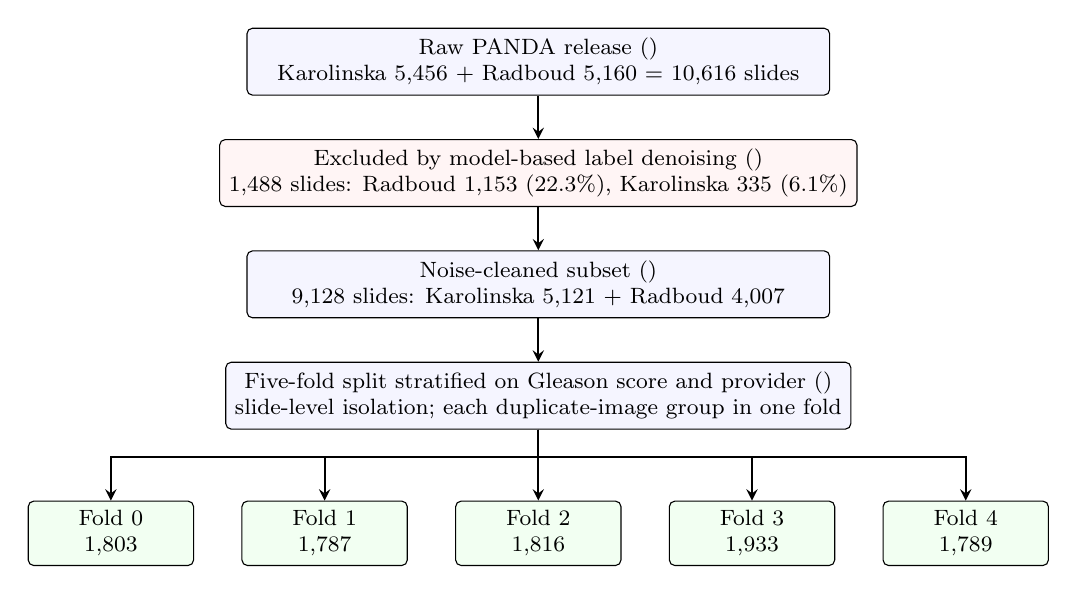
\begin{tikzpicture}[
  node distance=0.55cm and 0.6cm,
  every node/.style={font=\footnotesize},
  box/.style={draw, rectangle, rounded corners=2pt, minimum width=7.4cm,
              minimum height=0.85cm, align=center, fill=blue!4},
  excl/.style={draw, rectangle, rounded corners=2pt, minimum width=5.4cm,
              minimum height=0.65cm, align=center, fill=red!4},
  fold/.style={draw, rectangle, rounded corners=2pt, minimum width=2.1cm,
              minimum height=0.7cm, align=center, fill=green!5},
  arr/.style={-stealth, thick}
]
\node[box] (raw)
  {Raw PANDA release \citep{R009} \\ Karolinska 5{,}456 + Radboud 5{,}160 = 10{,}616 slides};
\node[excl, below=of raw] (excl)
  {Excluded by model-based label denoising \citep{R063} \\ 1,488 slides: Radboud 1,153 (22.3\%), Karolinska 335 (6.1\%)};
\node[box, below=of excl] (clean)
  {Noise-cleaned subset \citep{R063} \\ 9{,}128 slides: Karolinska 5,121 + Radboud 4,007};
\node[box, below=of clean] (split)
  {Five-fold split stratified on Gleason score and provider \citep{R063} \\
   slide-level isolation; each duplicate-image group in one fold};

\node[fold, below=0.9cm of split] (f2) {Fold 2 \\ 1{,}816};
\node[fold, left=of f2] (f1) {Fold 1 \\ 1{,}787};
\node[fold, left=of f1] (f0) {Fold 0 \\ 1{,}803};
\node[fold, right=of f2] (f3) {Fold 3 \\ 1{,}933};
\node[fold, right=of f3] (f4) {Fold 4 \\ 1{,}789};

\draw[arr] (raw) -- (excl);
\draw[arr] (excl) -- (clean);
\draw[arr] (clean) -- (split);
\draw[arr] (split.south) -- ++(0,-0.35) -| (f0.north);
\draw[arr] (split.south) -- ++(0,-0.35) -| (f1.north);
\draw[arr] (split.south) -- ++(0,-0.35) -| (f2.north);
\draw[arr] (split.south) -- ++(0,-0.35) -| (f3.north);
\draw[arr] (split.south) -- ++(0,-0.35) -| (f4.north);
\end{tikzpicture}
\end{document}
